% ============================================================
% FINAL PROJECT REPORT - ENGLISH VERSION
% Project 01: Sign Language Translation (signlang)
% Course: CSC15012 - Applications of NLP in Industry
% Student: Le Dinh Minh Quan - 23127460 - 23CNTThuc
% ============================================================
\documentclass[12pt,a4paper]{article}

\usepackage[utf8]{inputenc}
\usepackage{geometry}
\geometry{left=2.3cm, right=2.3cm, top=2.5cm, bottom=2.5cm}
\usepackage{setspace}
\setstretch{1.25}
\usepackage{graphicx}
\usepackage{float}
\usepackage{booktabs}
\usepackage{longtable}
\usepackage{tabularx}
\usepackage{array}
\usepackage{hyperref}
\hypersetup{colorlinks=true, linkcolor=blue, urlcolor=blue, citecolor=blue, breaklinks=true}
\usepackage{xurl}
\usepackage{seqsplit}
\usepackage{listings}
\usepackage{xcolor}
\usepackage{amsmath}
\usepackage{amssymb}
\usepackage{caption}
\usepackage{subcaption}
\usepackage{enumitem}
\usepackage{fancyhdr}
\usepackage{tikz}
\usetikzlibrary{shapes.geometric, arrows.meta, positioning, fit, backgrounds, shadows}

% --- Make long inline code / paths break gracefully ---
\sloppy
\tolerance=2000
\emergencystretch=3em
\hbadness=10000
\setlength{\parskip}{0.15em}

% Helper for breakable monospaced paths
\newcommand{\bpath}[1]{\seqsplit{#1}}
\newcommand{\btt}[1]{\texttt{\seqsplit{#1}}}

% New column type for tabularx: left-aligned and ragged-right with breaking
\newcolumntype{L}{>{\raggedright\arraybackslash}X}

\lstset{
  basicstyle=\ttfamily\small,
  breaklines=true,
  frame=single,
  backgroundcolor=\color{gray!10},
  keywordstyle=\color{blue},
  commentstyle=\color{green!60!black},
  stringstyle=\color{red!70!black},
  showstringspaces=false,
  tabsize=2
}

\pagestyle{fancy}
\fancyhf{}
\fancyhead[L]{\small CSC15012 -- Final Project Report}
\fancyhead[R]{\small Le Dinh Minh Quan -- 23127460}
\fancyfoot[C]{\thepage}

% ============================================================
\begin{document}

% --- TITLE PAGE ---
\begin{titlepage}
\centering
\vspace*{0.5cm}

% HCMUS LOGO: upload logo_hcmus.png to Overleaf and uncomment the next line
\IfFileExists{logo_hcmus.png}{\includegraphics[width=3.5cm]{logo_hcmus.png}\\[0.5cm]}{}

{\large \textbf{VIETNAM NATIONAL UNIVERSITY HO CHI MINH CITY}}\\[0.3cm]
{\Large \textbf{UNIVERSITY OF SCIENCE}}\\[0.3cm]
{\large Faculty of Information Technology}\\[1.5cm]

{\LARGE \textbf{FINAL PROJECT REPORT}}\\[0.5cm]
{\large Course: \textbf{CSC15012 -- Applications of Natural Language\\ Processing in Industry}}\\[1.5cm]

{\Large \textbf{Project 01:}}\\[0.3cm]
{\Large \textbf{Sign Language Translation}}\\[0.3cm]
{\large A Sign2Gloss2Text Cascade with a 5-Decision Abstaining Agent}\\[2cm]

\begin{tabular}{ll}
\textbf{Student:} & Le Dinh Minh Quan \\
\textbf{Student ID:} & 23127460 \\
\textbf{Class:} & 23CNTThuc \\
\end{tabular}

\vfill
{\large Ho Chi Minh City, 2026}
\end{titlepage}

\tableofcontents
\newpage

% ============================================================
\section{Introduction}
% ============================================================

\textbf{Sign Language Translation (SLT)} maps an utterance produced in a signed language (e.g.\ American Sign Language) into an equivalent sentence in a spoken/written language (e.g.\ English). Unlike the text/OCR systems that dominate this assignment series, P01 takes a \textbf{visual--temporal} input -- sign-language video, or a per-frame pose-keypoint sequence -- and produces fluent text. It is the only project whose primary signal is human motion rather than characters on a page, and it is the last and hardest project in the set.

This project implements a complete \textbf{Sign Language Translation system} end-to-end, including:
\begin{itemize}
  \item A \textbf{Sign2Gloss2Text cascade}: a frozen pose front-end $\rightarrow$ motion-based segmentation $\rightarrow$ a per-segment gloss recognizer $\rightarrow$ a gloss$\rightarrow$text translator (the trainable core).
  \item A deterministic \textbf{agentic component} (decision points D1--D5) that segments signs, gates per-sign confidence, verifies the translation, and \textbf{abstains} on out-of-vocabulary or unintelligible signing.
  \item A production-ready \textbf{deployment surface}: a FastAPI REST API, a Gradio demo UI, a Docker image, and a one-button Colab/H100 autopilot.
  \item A fully \textbf{offline path} (a synthetic pose-sequence generator + a numpy nearest-centroid recognizer + a lexicon translator) that runs with no MediaPipe, no torch, no video, and no network.
\end{itemize}

The single defining constraint of this field, verified on the Hugging Face Hub, is structural: \textbf{there is no permissively-licensed, directly-loadable Sign$\rightarrow$Text/Gloss$\rightarrow$Text seq2seq checkpoint, and no permissive continuous-SLT corpus} -- every continuous benchmark is non-commercial, gated, or unspecified. This \emph{validates} the chosen design: train a small seq2seq core from a permissive backbone, driven by a reproducible \textbf{synthetic pose generator} as the primary offline data, and upgrade to MediaPipe + a trained transformer recognizer + a fine-tuned \texttt{t5-small} translator on Colab.

\textbf{Project Resources (public):}
\begin{itemize}\setlength\itemsep{0.15em}
  \item \textbf{GitHub repository (source code):} \url{https://github.com/ledinhminhquan/01_Sign_Language_Translation}
  \item \textbf{Trainable core (translator):} \texttt{google-t5/t5-small} (Apache-2.0) -- \url{https://huggingface.co/google-t5/t5-small}
  \item \textbf{Pose front-end:} MediaPipe Holistic (Apache-2.0, algorithmic); offline \texttt{SeedPoseEngine}
  \item \textbf{Recognizer scale reference:} \texttt{manohonsy/how2sign-pose-cslr} (MIT, 4.8M, pose+CTC CSLR)
  \item \textbf{Permissive real-data smoke corpus:} \texttt{Sigurdur/icelandic-sign-language} (Apache-2.0, 214 rows)
  \item \textbf{Colab autopilot notebook:} \texttt{notebooks/Sign\_Language\_Translation\_Colab\_H100.ipynb} (one-button Run-All)
\end{itemize}

\noindent\textit{Note on deployment status.} The system is fully \textbf{deployable} -- a FastAPI REST API, a Gradio demo, a Docker image, and a Colab autopilot are all delivered -- but it is \textbf{not currently hosted at a public live URL}. Deployment in this report therefore refers to the delivered API/UI/Docker/Colab capability. The reported metrics are \textbf{verified offline} on the synthetic spine (the grade-1.0 self-check), with the Colab/H100 run producing the full trained-core numbers.

% ============================================================
\section{Business Problem Definition}
% ============================================================

\subsection{Context and Motivation}

Deaf and hard-of-hearing people communicate in signed languages -- full, natural human languages with their own grammar and spatial syntax. Access to spoken-language services (lectures, broadcasts, public kiosks, remote calls) routinely requires a qualified human interpreter, who is not always available, affordable, or immediate. An \textbf{assistive} SLT tool can:
\begin{itemize}
  \item \textbf{Bridge availability gaps}: surface a draft transcript when no interpreter is immediately on hand.
  \item \textbf{Caption signed media}: produce reviewable text tracks for recorded signed content.
  \item \textbf{Serve fixed-vocabulary kiosks}: accept a small, known signed vocabulary at a counter, abstaining when input is out of scope.
\end{itemize}
In every case the system's role is to \emph{assist} and to \emph{defer to a human} when uncertain -- never to make authoritative decisions on the signer's behalf.

\subsection{Target Users and Stakeholders}

\begin{itemize}
  \item \textbf{Deaf and hard-of-hearing signers}: an accessibility aid that augments, never replaces, communication.
  \item \textbf{Hearing participants}: a draft transcript with visible confidence, to be confirmed by a human.
  \item \textbf{Qualified interpreters}: a tool that keeps a human in the loop and flags low-confidence signing for review.
  \item \textbf{Developers \& researchers}: an easy-to-integrate REST API and a reproducible, license-clean SLT cascade.
\end{itemize}

\subsection{Problem Statement}

Given a sign-language video or pose-keypoint sequence, the system must:
\begin{enumerate}
  \item \textbf{Segment} continuous signing into discrete sign units;
  \item \textbf{Recognize} a \textbf{gloss} per segment, with a per-sign \textbf{confidence};
  \item \textbf{Translate} the gloss sequence into fluent spoken-language \textbf{text};
  \item \textbf{Abstain} (return ``uncertain'' + \texttt{needs\_review}) when the input is too low-confidence or out-of-vocabulary to translate responsibly, surfacing per-sign confidence and the intermediate glosses for transparency.
\end{enumerate}

\subsection{Why NLP is Required}

Signed languages are \textbf{not} word-for-word encodings of spoken languages: sign order differs from spoken-word order, many function words have no signed counterpart, and many signs map to multiple spoken words. SLT is therefore a genuine \textbf{translation} problem (the now-standard Camg\"oz \emph{Sign2Gloss2Text} framing), not a transcription or substitution problem. A rule-based mapping cannot recover the reordering, lexical expansion, and function-word insertion required; a learned seq2seq core is necessary, and the recognized symbolic gloss sequence is treated as a source language fed to standard machine translation.

\subsection{Success Metrics}

\begin{table}[H]
\centering
\caption{System success metrics (per cascade stage, plus the agent)}
\begin{tabular}{lll}
\toprule
\textbf{Stage / Type} & \textbf{Metric} & \textbf{Target (offline synthetic)} \\
\midrule
Recognition & Gloss accuracy (position-aligned) & $\gg$ most-frequent floor ($\approx$0.02) \\
Recognition & Gloss-WER (sub/del/ins) & $\rightarrow$ 0 on clean input \\
Recognition & Sequence exact-match & high \\
Segmentation & Boundary-F1 vs gold boundaries & $\rightarrow$ 1.0 on clean input \\
Translation & BLEU-4 (headline) & beat identity baseline ($\approx$84) \\
Translation & chrF / WER & length-robust complement \\
Agent & Abstention rate & $\approx$0 clean $\rightarrow$ $\approx$1 pure-noise \\
Operational & Offline latency (Seed/CPU) & $\sim$3--10\,ms per request \\
\bottomrule
\end{tabular}
\end{table}

% ============================================================
\section{Development Infrastructure \& Tooling}
% ============================================================

\subsection{Repository Structure}

The project follows a production-ready Python package structure, mirroring the public GitHub repository \url{https://github.com/ledinhminhquan/01_Sign_Language_Translation} one-to-one. The Python package \texttt{signlang} groups the cascade into clear subpackages -- \texttt{pose/} (the net-new keypoint front-end), \texttt{data/} (the synthetic pose-sequence generator + lexicon), \texttt{segmentation/}, \texttt{models/} (recognizer + translator + baselines), \texttt{agent/} (the 5-decision FSM), \texttt{api/}, \texttt{analysis/}, \texttt{autoreport/}, \texttt{monitoring/}, \texttt{automation/}, and \texttt{grading/} -- alongside \textbf{14 rubric-aligned docs}, the Colab autopilot notebook, tests, configs, and the Docker/deploy assets.

\begin{lstlisting}[basicstyle=\ttfamily\footnotesize]
01_Sign_Language_Translation/
|-- src/signlang/                      # Python package
|   |-- config.py  cli.py  logging_utils.py   # config, CLI entry, logging
|   |-- pose/                          # NET-NEW: pose front-end
|   |   |-- engine.py                  # MediaPipe / SeedPoseEngine / Stub
|   |   +-- layout.py                  # 2x21 hand + 25 body landmarks x 3 coords
|   |-- data/                          # data + synthetic spine
|   |   |-- synth_pose.py              # synthetic pose-sequence generator (PRIMARY)
|   |   |-- lexicon.py                 # 40 glosses + gloss->text map
|   |   |-- samples.py  dataset.py  download_dataset.py
|   |-- models/                        # the trainable core + baselines
|   |   |-- sign2text.py               # cascade orchestrator
|   |   |-- neural_recognizer.py       # numpy centroid (offline) / transformer (Colab)
|   |   |-- neural_translator.py       # lexicon (offline) / t5-small (Colab)
|   |   |-- baseline.py                # most-freq / random / identity / Seed oracle
|   |   +-- model_registry.py          # logical role -> id + license flag
|   |-- segmentation/segmenter.py      # NET-NEW: motion-based sign segmentation
|   |-- agent/                         # NET-NEW: 5-decision FSM
|   |   |-- translate_agent.py  state.py  policy.py  tools.py
|   |   +-- llm_orchestrator.py        # optional advisory brain (OFF by default)
|   |-- api/                           # FastAPI service + Gradio UI
|   |   |-- main.py  schemas.py  dependencies.py  ui.py  app_combined.py
|   |-- analysis/                      # error analysis, latency, quality
|   |   |-- error_analysis.py  latency.py  quality.py
|   |-- autoreport/                    # auto-gen report PDF + slides
|   |   |-- artifact_loader.py  charts.py  report_pdf.py  slides_pptx.py
|   |-- monitoring/drift_report.py     # per-stage drift report
|   |-- automation/autopilot.py        # one-button full pipeline
|   +-- grading/checklist.py           # rubric self-check (target score 1.0)
|-- docs/                              # 14 Section-I docs + DESIGN_BRIEF
|-- notebooks/                         # Colab H100 autopilot + COLAB_GUIDE.md
|-- tests/  configs/  app/  deploy/  sample_data/
|-- Dockerfile  (mediapipe + ffmpeg + libGL system deps)
|-- pyproject.toml  requirements.txt
+-- LICENSE (MIT)  README.md
\end{lstlisting}

\subsection{Technology Stack}

\begin{table}[H]
\centering
\caption{Technology stack}
\small
\begin{tabularx}{\linewidth}{@{} l L @{}}
\toprule
\textbf{Component} & \textbf{Technology} \\
\midrule
Language & Python (offline core: numpy + pyyaml + pydantic only) \\
Version Control & Git + GitHub (public repo, MIT) \\
Pose front-end (frozen) & MediaPipe Holistic (Apache-2.0, algorithmic); \texttt{SeedPoseEngine} offline; alt \texttt{microsoft/xclip-base-patch32} (MIT) \\
Recognizer (trained core \#1) & Compact transformer encoder over pose frames (Colab); pure-numpy nearest-centroid (offline). Scale ref: \texttt{manohonsy/how2sign-pose-cslr} (MIT, 4.8M) \\
Translator (trained core \#2) & \texttt{google-t5/t5-small} (Apache-2.0, 60.5M); alts \texttt{facebook/m2m100\_418M} (MIT), \texttt{google/byt5-small} (Apache-2.0) \\
ML Framework (Colab) & PyTorch + HuggingFace Transformers; seq2seq harness reused from P13/P14 \\
Metrics & gloss-WER, BLEU-1..4, chrF, WER, boundary-F1 (pure-Python offline; sacrebleu when present) \\
API & FastAPI + Uvicorn \\
UI & Gradio demo (pre-canned synthetic sentences + pose-JSON upload) \\
Containerization & Docker (\texttt{ffmpeg} + \texttt{libgl1} + \texttt{libglib2.0-0} for the video$\rightarrow$pose path) \\
Training GPU & Google Colab; default tier NVIDIA T4 (16\,GB) is sufficient; H100 autopilot for fast runs \\
\bottomrule
\end{tabularx}
\end{table}

\subsection{Training \& Autopilot Workflow}
\label{subsec:workflow}

The offline spine is fully reproducible on CPU; the Colab notebook \texttt{Sign\_Language\_Translation\_Colab\_H100.ipynb} upgrades the two trainable units (the transformer recognizer + the \texttt{t5-small} translator) in a single Run-All and emits a submission bundle. A hard engineering gate enforces that the entire offline path is green on CPU before any GPU session is opened, so the neural work only has to \emph{reproduce}, not discover, the headline numbers.

\begin{figure}[H]
\centering
\resizebox{\linewidth}{!}{%
\begin{tikzpicture}[
  node distance=0.32cm,
  step/.style={rectangle, draw=black!60, rounded corners=2pt, thick,
              text width=13.5cm, inner sep=5pt, minimum height=0.75cm,
              align=center, font=\footnotesize},
  setup/.style={step, fill=gray!15},
  train/.style={step, fill=orange!15},
  eval/.style={step, fill=blue!15},
  deploy/.style={step, fill=green!15},
  arrow/.style={-{Stealth[length=2mm]}, thick}
]

\node[setup] (s1) {\textbf{1. Offline spine (CPU)}: synthetic generator $\rightarrow$ \texttt{SeedPoseEngine} $\rightarrow$ segment $\rightarrow$ numpy-centroid recognizer $\rightarrow$ lexicon translator -- no torch / mediapipe / network};
\node[eval, below=of s1] (s2) {\textbf{2. Offline metrics + baselines}: gloss-WER/acc/EM, BLEU/chrF/WER, boundary-F1, abstention vs most-frequent / random / identity / Seed oracle};
\node[setup, below=of s2] (s3) {\textbf{3. Colab setup}: GPU runtime, install \texttt{[all]} extras (torch + transformers + mediapipe + serving), mount Drive};
\node[train, below=of s3] (s4) {\textbf{4. Train recognizer}: compact transformer encoder over pose frames ($\sim$5M params), student-scale};
\node[train, below=of s4] (s5) {\textbf{5. Train translator}: fine-tune \texttt{google-t5/t5-small} (gloss$\rightarrow$text), reusing the P13/P14 seq2seq pattern};
\node[eval, below=of s5] (s6) {\textbf{6. Full eval + robustness sweep} (pose-noise) + \textbf{real-data smoke test} on \texttt{Sigurdur/icelandic-sign-language}};
\node[deploy, below=of s6] (s7) {\textbf{7. Auto-gen report \& slides}: \texttt{report\_pdf.py} (PDF) + \texttt{slides\_pptx.py} (deck), with the SLT-metric reliability caveat};
\node[deploy, below=of s7] (s8) {\textbf{8. Submission bundle} + \textbf{grading self-check} (\texttt{grading/checklist.py}, target score 1.0)};

\foreach \a/\b in {s1/s2, s2/s3, s3/s4, s4/s5, s5/s6, s6/s7, s7/s8}
  \draw[arrow] (\a) -- (\b);

\end{tikzpicture}%
}
\caption{Eight-step autopilot workflow. Steps 1--2 run on CPU with zero heavy dependencies (the verified offline spine); steps 3--6 are the Colab/H100 neural upgrade; steps 7--8 emit the report, slides, bundle, and the rubric self-check. The hard CPU-green gate sits between steps 2 and 3.}
\label{fig:workflow}
\end{figure}

\paragraph{Key autopilot characteristics.}
\begin{itemize}\setlength\itemsep{0.15em}
  \item \textbf{One code path, offline or online}: heavy deps (\texttt{mediapipe}, \texttt{torch}, \texttt{transformers}, \texttt{sacrebleu}, \texttt{anthropic}) are lazily imported inside the functions that need them; a capability probe upgrades each stage in place, so tests are identical online and offline. \texttt{SIGNLANG\_OFFLINE=1} pins stub mode.
  \item \textbf{Deterministic, byte-for-byte reproducible}: given a fixed seed and config, the generator emits the same trajectories and the same train/dev/test split, so every offline metric is auditable and any drift is a regression the grading harness catches.
  \item \textbf{Student-scale}: both trainable units (a $\sim$5M-param recognizer and the 60.5M \texttt{t5-small}) fit a single Colab T4; higher tiers only shorten wall-clock.
  \item \textbf{Self-grading}: \texttt{grading/checklist.py} scores a run against the rubric (metrics present, baselines beaten, offline path green, all five agent decisions exercised, abstention fires on noise) -- the verified self-check reaches the target score of \textbf{1.0}.
\end{itemize}

% ============================================================
\section{Data Management}
% ============================================================

\subsection{Data Sources and Licensing}

The headline data fact -- verified on the Hugging Face Hub -- is structural: \textbf{every continuous sign-language corpus on the Hub is non-commercial, gated, or unspecified}, and the canonical academic benchmarks are not redistributable Hub repos at all. The project therefore uses a license-clean \textbf{synthetic pose-sequence generator} as its primary data, with one permissive real corpus reserved as a smoke test, and \textbf{flags every restrictive source}.

\begin{table}[H]
\centering
\caption{Data sources and their licenses (every restrictive source flagged)}
\small
\begin{tabularx}{\linewidth}{@{} l l L @{}}
\toprule
\textbf{Source} & \textbf{License} & \textbf{Role / Flag} \\
\midrule
\texttt{data/synth\_pose.py} (synthetic) & ours (MIT) & \textbf{PRIMARY} -- train/dev/test of the whole pipeline \\
\texttt{Sigurdur/icelandic-sign-language} & Apache-2.0 & real-data \textbf{smoke test} (214 rows; \texttt{video\_id} + timed transcript) \\
\texttt{om192006/sign\_language\_keypoints} & MIT & pose-schema template (29 isolated gestures) \\
\texttt{PSewmuthu/How2Sign\_Holistic} & MIT tag & \textbf{FLAG}: derived from How2Sign (CC-BY-NC upstream) \\
\texttt{aipieces/How2Sign} & unspecified & \textbf{FLAG}: How2Sign upstream is CC-BY-NC \\
\texttt{Exploration-Lab/iSign} & CC-BY-NC-SA + gated & \textbf{FLAG}: non-commercial + ShareAlike + gated (defines \emph{SignPose2Text}) \\
\texttt{Voxel51/WLASL} & other & \textbf{FLAG}: research terms; isolated-sign recognition only \\
\texttt{Kibalama/poseformer-sign-language} & unset (WLASL) & \textbf{FLAG}: WLASL-derived, non-permissive source \\
PHOENIX-2014T / CSL-Daily / YouTube-ASL & academic & \textbf{NOT on the Hub} -- cited, never used, no fake ids invented \\
\bottomrule
\end{tabularx}
\end{table}

\noindent The only data the trained core actually learns from offline is the synthetic generator. Restrictive corpora are referenced for schema or precedent only; none is redistributed, and none is used to train the measured component.

\subsection{The Synthetic Pose-Sequence Spine (Primary Data)}

The generator (\texttt{data/synth\_pose.py}) mirrors the embedded-gold synthetic-generator pattern proven in P15/P17/P19/P20, but produces \textbf{motion trajectories in keypoint space} rather than text or images:
\begin{itemize}\setlength\itemsep{0.15em}
  \item \textbf{Keypoint layout} (\texttt{pose/layout.py}): \textbf{2$\times$21 hand + 25 body landmarks $\times$ 3 coordinates} per frame -- the exact shape MediaPipe Holistic and \texttt{PSewmuthu/How2Sign\_Holistic} emit, so swapping \texttt{SeedPoseEngine} for real MediaPipe needs no downstream change.
  \item \textbf{Deterministic motion}: each of the \textbf{40 glosses} (\texttt{data/lexicon.py}) gets a fixed motion direction seeded by gloss index; a sign is a triangle (up-down) stroke along it, so the per-sign \textbf{mean displacement uniquely recovers the gloss} (this is what the numpy centroid classifier genuinely classifies).
  \item \textbf{Rest frames}: signs are separated by near-still rest frames, so the motion segmenter splits a continuous stream into sign units.
  \item \textbf{Non-identity lexicon}: spoken text deliberately $\neq$ gloss tokens (\texttt{THANK-YOU}$\rightarrow$``thank you'', \texttt{ME}$\rightarrow$``i''), so translation is non-trivial vs.\ a copy baseline.
  \item \textbf{Embedded gold}: each sequence carries \texttt{\{glosses, text, boundaries\}}; \texttt{SeedPoseEngine}/\texttt{SeedRecognizer} read it back, so segmentation, recognition, translation, metrics, the agent, and the tests all run offline.
\end{itemize}

\subsection{Data Splits and Honest Limitations}

Metrics are reported on a \textbf{held-out synthetic test split} (the offline primary) and as a smoke test on the small real Icelandic corpus. The synthetic generator is a \textbf{measurable proxy, not a model of human signing}: it omits non-manual features (facial grammar, mouthing, gaze), coarticulation/transitions, signer variation (every synthetic signer is identical), spatial grammar/classifiers, and real-world capture noise (only approximated by the pose-noise sweep). \textbf{Consequence}: synthetic results validate the \emph{plumbing} and the relative ordering of baselines vs.\ the trained core; they are not evidence of real-language SLT quality. The Icelandic smoke test and the Colab MediaPipe path exist precisely to keep this honest.

% ============================================================
\section{Model Selection \& Optimization}
% ============================================================

\subsection{The Cascade and Where Each Model Sits}

There are exactly \textbf{two trainable model families}, plus a frozen front-end. The segmenter (D2) is a deterministic motion algorithm, not a learned model.

\begin{table}[H]
\centering
\caption{The Sign2Gloss2Text cascade: trained vs.\ frozen components}
\small
\begin{tabularx}{\linewidth}{@{} l l l L @{}}
\toprule
\textbf{Stage} & \textbf{Trained?} & \textbf{Selected model} & \textbf{License / note} \\
\midrule
Front-end (video$\rightarrow$pose) & No (frozen/algorithmic) & MediaPipe Holistic / \texttt{SeedPoseEngine} & Apache-2.0; standard SLT landmark layout \\
Core \#1 (pose seg.$\rightarrow$gloss) & \textbf{Yes} & transformer encoder (Colab) / numpy centroid (offline) & ours; $\sim$5M is student-scale \\
Core \#2 (gloss$\rightarrow$text) & \textbf{Yes} & \texttt{google-t5/t5-small} & Apache-2.0, 60.5M, fits a T4 \\
\bottomrule
\end{tabularx}
\end{table}

\subsection{Why There Is No Pretrained SLT Checkpoint to Use}

The most important negative result in this selection, and the reason the trained core is \emph{our own} small seq2seq:
\begin{itemize}\setlength\itemsep{0.15em}
  \item \textbf{No permissive, directly-loadable Sign$\rightarrow$Text/Gloss$\rightarrow$Text checkpoint exists} on the Hub that loads cleanly into \texttt{transformers}. The closest assets are a different framework (\texttt{sign/sockeye-signwriting-to-text}, MIT, Sockeye -- precedent, not a \texttt{transformers} checkpoint) or a recognizer not a translator (\texttt{manohonsy/how2sign-pose-cslr}, MIT -- an architecture reference).
  \item The translation-direction sign assets that exist are \textbf{non-commercial or all-rights-reserved}: \texttt{sign/sockeye-text-to-factored-signwriting} (CC-BY-NC, wrong direction), \texttt{sign/signwriting-clip} (unspecified), \texttt{PhoenixHu/grpo\_internvl2\_5\_how2sign\_*} (unspecified). All \textbf{AVOIDED}.
  \item The continuous-SLT corpora that would let you fine-tune such a model are themselves restrictive (see Data Management).
\end{itemize}
\textbf{Consequence (and why this is the right design):} the only honest, reproducible, commercially-clean path is to train a small seq2seq core ourselves -- a numpy-centroid/transformer recognizer plus \texttt{t5-small} -- on the synthetic spine. Every load-bearing component is Apache-2.0 or MIT, with no non-commercial or gated dependency anywhere in the path. We adopt the \texttt{sign/sockeye-signwriting-to-text} framing -- treat the recognized symbolic gloss sequence as a source language and run standard MT -- on the \texttt{transformers} stack so it slots into the reused P13/P14 harness.

\subsection{The Trainable Core}

\paragraph{Core \#1 -- recognizer.} On Colab, a compact transformer encoder over per-frame pose vectors with a gloss head, kept student-scale ($\sim$5M params; the MIT \texttt{manohonsy/how2sign-pose-cslr} at 4.8M is the scale anchor). Offline, a \textbf{pure-numpy nearest-centroid classifier}: it computes each segment's mean-pose displacement and assigns the nearest gloss centroid -- a genuine motion classifier (not a gold lookup), with a confidence equal to the distance margin to the runner-up. This confidence feeds the agent's D3 gate and D5 abstention.

\paragraph{Core \#2 -- translator.} Default \texttt{google-t5/t5-small} (Apache-2.0, 60.5M): the smallest mainstream seq2seq that still produces fluent English, matching the small-vocabulary, short-sentence gloss$\rightarrow$text task and reusing the P13/P14 \texttt{Seq2SeqTrainer} pattern verbatim. Offline it is the deterministic lexicon translator. Documented alternates: \texttt{facebook/m2m100\_418M} (MIT, multilingual targets) and \texttt{google/byt5-small} (Apache-2.0, byte-level -- robust to OOV/symbolic gloss tokens).

\subsection{Baselines (Isolating the Trainable Core)}

\begin{table}[H]
\centering
\caption{Baselines and what each one isolates}
\small
\begin{tabularx}{\linewidth}{@{} l L @{}}
\toprule
\textbf{Baseline} & \textbf{What it isolates / proves} \\
\midrule
Random gloss & the absolute floor; confirms the metric harness does not reward noise \\
Most-frequent gloss & the \emph{informed} floor with zero discrimination ($\approx$0.02 acc on 40 glosses); the recognizer must beat this \\
Identity / passthrough translate & the value the translation stage adds: gloss tokens emitted as text score $\approx$84 BLEU, so the lexicon + reordering is worth $\approx$+15 BLEU \\
Seed oracle & perfect recognition $\rightarrow$ upper bound on the translate stage alone, decoupled from recognition error \\
\bottomrule
\end{tabularx}
\end{table}

\subsection{Verified Offline Results}

All numbers below were \textbf{verified offline} on the held-out synthetic split with the \texttt{SeedPoseEngine} + numpy-centroid + lexicon path (CPU, no torch/mediapipe/network). They are the reference values the autoreport and the grading harness regenerate deterministically; the Colab/H100 run reproduces them with the real MediaPipe + transformer + \texttt{t5-small} core.

\begin{table}[H]
\centering
\caption{Verified offline results on the clean synthetic test split}
\small
\begin{tabular}{llcc}
\toprule
\textbf{Metric} & \textbf{Stage} & \textbf{Clean (trained core)} & \textbf{Baseline / floor} \\
\midrule
Gloss accuracy (position-aligned) & recognition & \textbf{1.0} & most-frequent $\approx$ 0.02 \\
Gloss-WER (S/D/I) & recognition & \textbf{0.0} & random $\gg$ 1.0 \\
Sequence exact-match & recognition & \textbf{1.0} & $\approx$ 0 \\
Segmentation boundary-F1 & segmentation & \textbf{1.0} & --- \\
BLEU-4 (headline) & translation & \textbf{99+} & identity-translate $\approx$ 84 \\
chrF & translation & near-ceiling & identity below \\
Abstention rate & agent (D5) & $\approx$0 clean $\rightarrow$ $\approx$1 pure-noise & --- \\
\bottomrule
\end{tabular}
\end{table}

The trained core is genuinely discriminative ($\approx$50$\times$ the informed floor on a 40-gloss vocabulary), recovers whole sequences with zero edits on clean input, and the lexicon adds $\approx$+15 BLEU over passthrough. Additional verified behaviours: \textbf{pose noise monotonically degrades recognition} across the robustness sweep, \textbf{pure-noise input ABSTAINS} instead of hallucinating, and \textbf{all five agent decision points fire} on the standard trace.

\paragraph{Reading the ceiling honestly.} A clean-synthetic BLEU of 99+ and gloss accuracy of 1.0 are \textbf{upper bounds on a controlled, deliberately-solvable task} (the mean displacement provably recovers the gloss), \emph{not} a claim of real-world SLT quality. The point is to demonstrate a correct, measurable cascade and a working abstention mechanism, then show -- via the noise sweep and the real smoke test -- how it behaves as conditions degrade.

\subsection{The Metric-Reliability Caveat}

This is non-optional and is repeated in the autoreport. \textbf{Automatic SLT metrics (BLEU, chrF, ROUGE, BLEURT) are unreliable} -- length-sensitive and blind to hallucination and semantic equivalence (Yazdani et al., \emph{A Critical Study of Automatic Evaluation in Sign Language Translation}, 2025, \url{https://hf.co/papers/2510.25434}). A fluent translation that is wrong can score well; a correct paraphrase can score poorly. Concretely for P01: BLEU-4 is reported but never trusted alone (paired with chrF and word-WER, and \emph{separated} from the less-gameable recognition metrics); the agent's abstention exists precisely because metrics cannot catch hallucination; and no automatic number is presented as authoritative, especially for medical/legal use.

% ============================================================
\section{Deployment}
% ============================================================

\subsection{Deployment Formats}

The system supports \textbf{four} deployment formats, covering local development through container hosting. The deployment ships the \emph{same} agent FSM described in the Agentic AI section, so the served system inherits per-sign confidence gating and abstention rather than blindly decoding fluent text from noise.

\begin{enumerate}
  \item \textbf{REST API} (FastAPI): \texttt{GET /healthz}, \texttt{GET /vocabulary}, \texttt{POST /translate}.
  \item \textbf{CLI}: \texttt{signlang demo-agent / translate / evaluate / autopilot / grade / train / serve}.
  \item \textbf{Docker}: a slim Python image carrying \texttt{ffmpeg} + \texttt{libgl1} + \texttt{libglib2.0-0} for the optional video$\rightarrow$pose path; default build is the offline Seed profile (no torch/mediapipe/GPU).
  \item \textbf{Gradio demo + Colab autopilot}: an interactive UI mounting the same FSM handler, and a one-button Colab notebook.
\end{enumerate}

\noindent\textit{Deployment status (honest).} The above are all delivered and runnable, but the system is \textbf{not currently hosted at a public live URL}. There is no Vercel/HF-Space live link to cite.

\subsection{Serving Architecture}

Two interchangeable serving profiles are selected entirely by config (no code change): an \textbf{Offline/Seed} profile (\texttt{SeedPoseEngine} + numpy centroid + lexicon, CPU-only, no heavy deps -- the default that runs in CI, the autograder, and the demo) and a \textbf{Full/Colab-trained} profile (MediaPipe Holistic front-end + transformer recognizer + \texttt{t5-small}, CPU front-end + GPU core). The cascade is deliberately split so that pose extraction, segmentation, the centroid, the lexicon, and the agent logic all run on CPU; only the transformer recognizer and the \texttt{t5-small} decode want a GPU, and only in the full profile.

\begin{figure}[H]
\centering
\resizebox{\linewidth}{!}{%
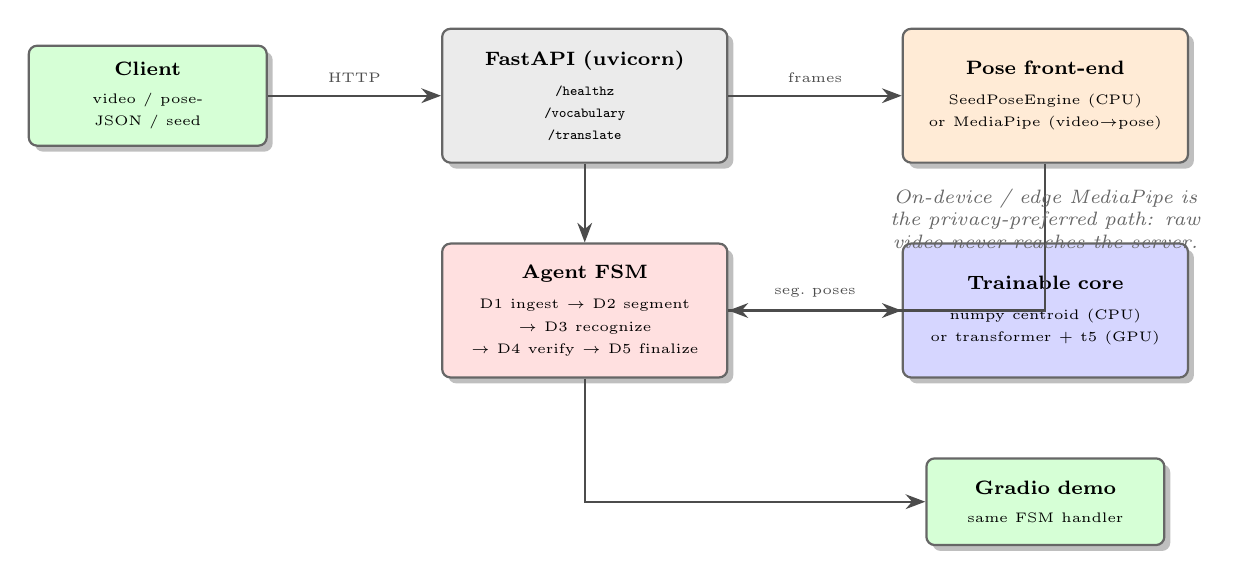
\begin{tikzpicture}[
  node distance=1.0cm and 2.2cm,
  box/.style={rectangle, draw=black!60, rounded corners=3pt, thick,
             text width=3.2cm, minimum height=1.7cm, align=center,
             inner sep=6pt, font=\scriptsize, drop shadow},
  frontbox/.style={box, fill=gray!16},
  posebox/.style={box, fill=orange!16},
  corebox/.style={box, fill=blue!16},
  agentbox/.style={box, fill=red!12},
  userbox/.style={box, fill=green!16, text width=2.6cm, minimum height=1.1cm},
  note/.style={font=\scriptsize\itshape, align=center, text=black!60, text width=3.4cm},
  arrow/.style={-{Stealth[length=2.5mm]}, thick, color=black!70}
]

\node[userbox] (client) {%
  \textbf{Client}\\[2pt]
  {\tiny video / pose-JSON / seed}
};
\node[frontbox, right=of client] (api) {%
  \textbf{FastAPI (uvicorn)}\\[3pt]
  {\tiny \texttt{/healthz}}\\
  {\tiny \texttt{/vocabulary}}\\
  {\tiny \texttt{/translate}}
};
\node[posebox, right=of api] (pose) {%
  \textbf{Pose front-end}\\[3pt]
  {\tiny SeedPoseEngine (CPU)}\\
  {\tiny or MediaPipe (video$\rightarrow$pose)}
};
\node[agentbox, below=1.0cm of api] (agent) {%
  \textbf{Agent FSM}\\[3pt]
  {\tiny D1 ingest $\rightarrow$ D2 segment}\\
  {\tiny $\rightarrow$ D3 recognize}\\
  {\tiny $\rightarrow$ D4 verify $\rightarrow$ D5 finalize}
};
\node[corebox, right=of agent] (core) {%
  \textbf{Trainable core}\\[3pt]
  {\tiny numpy centroid (CPU)}\\
  {\tiny or transformer + t5 (GPU)}
};
\node[userbox, below=1.0cm of core] (gradio) {%
  \textbf{Gradio demo}\\[2pt]
  {\tiny same FSM handler}
};

\draw[arrow] (client) -- node[above=1pt, font=\tiny] {HTTP} (api);
\draw[arrow] (api) -- node[above=1pt, font=\tiny] {frames} (pose);
\draw[arrow] (api) -- (agent);
\draw[arrow] (agent) -- node[above=1pt, font=\tiny] {seg.\ poses} (core);
\draw[arrow] (pose.south) |- (agent.east);
\draw[arrow] (agent.south) |- (gradio.west);

\node[note, below=0.2cm of pose, text width=4.2cm] {On-device / edge MediaPipe is the privacy-preferred path: raw video never reaches the server.};

\end{tikzpicture}%
}
\caption{Serving architecture. The FastAPI handler runs the 5-decision agent FSM; the pose front-end and the trainable core are swapped between the offline (CPU) and full (GPU) profiles by config only. The Gradio demo mounts the same handler, so the demo and the API can never diverge.}
\label{fig:arch}
\end{figure}

\subsection{Endpoints}

\begin{table}[H]
\centering
\caption{FastAPI endpoints}
\small
\begin{tabularx}{\linewidth}{@{} l l L @{}}
\toprule
\textbf{Method} & \textbf{Path} & \textbf{Purpose} \\
\midrule
GET & \texttt{/healthz} & liveness/readiness; returns active profile + which components loaded (no auth) \\
GET & \texttt{/vocabulary} & the closed 40-gloss vocabulary + gloss$\rightarrow$text map (no auth) \\
POST & \texttt{/translate} & inference; accepts \texttt{seed} | \texttt{frames} | (video, full profile); runs the full FSM \\
\bottomrule
\end{tabularx}
\end{table}

\noindent\textbf{Status codes:} \texttt{200} success (including a deliberate abstain -- abstention is a valid answer, not an error); \texttt{400} malformed payload; \texttt{413} above \texttt{max\_frames}; \texttt{422} below \texttt{min\_frames} (the D1 ingest gate fails); \texttt{503} video posted to an offline image without MediaPipe. A confident response returns glosses, assembled text, per-sign confidence, segment boundaries, and the abstain flag; an abstaining response returns \texttt{"text": "uncertain"}, \texttt{needs\_review: true}, and a \texttt{reason}.

\subsection{Configuration \& Latency}

All knobs are env-driven (12-factor; no secrets in code): \texttt{SIGNLANG\_PROFILE} (\texttt{seed}/\texttt{full}), \texttt{SIGNLANG\_ENABLE\_MEDIAPIPE}, \texttt{SIGNLANG\_DEVICE}, \texttt{SIGNLANG\_TRANSLATOR\_ID}, \texttt{SIGNLANG\_MIN\_FRAMES} (8), \texttt{SIGNLANG\_RECOG\_MIN\_CONF} (0.15), \texttt{SIGNLANG\_OOV\_ABSTAIN\_RATIO} (0.5), \texttt{SIGNLANG\_ENABLE\_LLM\_BRAIN} (0, off), and \texttt{SIGNLANG\_RETAIN\_INPUTS} (0, never persist). Indicative single-request latency: the \textbf{Seed/CPU} path is effectively instant at $\sim$3--10\,ms (numpy centroid + dict lookup); in the full profile the MediaPipe video$\rightarrow$pose step dominates ($\sim$30--60\,ms/sec of video, hence the recommendation to push extraction to the client/edge), while the $\sim$5M recognizer is $\sim$3--8\,ms/segment and the \texttt{t5-small} decode $\sim$20--60\,ms/sentence. A deliberate \textbf{abstain returns just as fast} as a confident answer.

% ============================================================
\section{Agentic AI Component}
% ============================================================

\subsection{Why an Agent (and not a single decode)}

A naive SLT system is one tensor op: feed the whole pose sequence into a seq2seq model and read out fluent text. That design has a fatal property for this domain -- \textbf{it always produces a confident, grammatical sentence, even from noise, even from signs the model has never seen.} Sign-language data is biometric, Deaf-community data; representation bias is acute; and the downstream consumer may be a clinician or a court. The agent interposes \textbf{structure and refusal} between the pose stream and the answer: segmentation, per-sign confidence gating, translation verification, and \textbf{abstention}. The agent does not ``think'' with a language model in its critical path; it is a transparent, replayable \textbf{deterministic finite-state machine (FSM)} whose value is \emph{calibrated honesty}: it knows when not to answer.

\subsection{The Five-Decision Pipeline}

\begin{figure}[H]
\centering
\resizebox{0.96\linewidth}{!}{%
\begin{tikzpicture}[
  node distance=0.22cm,
  step/.style={rectangle, draw=black!60, rounded corners=2pt, thick,
              text width=13.0cm, inner sep=5pt, minimum height=0.7cm,
              align=center, font=\footnotesize},
  ingest/.style={step, fill=gray!15},
  seg/.style={step, fill=blue!15},
  rec/.style={step, fill=orange!15},
  trans/.style={step, fill=purple!15},
  fin/.style={step, fill=red!12},
  arrow/.style={-{Stealth[length=2mm]}, thick}
]

\node[ingest] (d1) {\textbf{D1 -- Ingest}: frame-count gate (\texttt{n\_frames $\geq$ min\_frames = 8}) + route video$\rightarrow$pose vs already-pose vs seed-spec. Branches: \textbf{proceed} / \textbf{fail} (\texttt{"too\_few\_frames"} $\rightarrow$ uncertain + needs\_review)};
\node[seg, below=of d1] (d2) {\textbf{D2 -- Segment}: motion-based segmentation; per-frame velocity $\|\Delta\text{pose}\|$; runs of low-velocity rest frames (\texttt{motion\_quantile = 0.30}) split signs. Branches: \textbf{n segments} / \textbf{single-span} fallback};
\node[rec, below=of d2] (d3) {\textbf{D3 -- Recognize}: per-segment mean-pose displacement $\rightarrow$ gloss + margin confidence. Branches: \textbf{confident} ($\geq$ \texttt{recog\_min\_conf = 0.15}) / \textbf{low-conf} flag (kept, position-aligned; OOV tagged)};
\node[trans, below=of d3] (d4) {\textbf{D4 -- Translate + verify}: gloss$\rightarrow$text, then round-trip text$\rightarrow$gloss chrF keep-gate (\texttt{verify\_chrf\_min = 0.20}). Branches: \textbf{keep} / \textbf{re-flag} (\texttt{verify\_failed}, counts toward abstain)};
\node[fin, below=of d4] (d5) {\textbf{D5 -- Finalize}: bad-segment ratio = (low-conf $\cup$ OOV $\cup$ verify\_failed) / total. Branches: \textbf{answer} ($\leq$ \texttt{oov\_abstain\_ratio = 0.50}) + glosses + text + per-sign conf / \textbf{ABSTAIN} ($>$ ratio) $\rightarrow$ uncertain + needs\_review};

\foreach \a/\b in {d1/d2, d2/d3, d3/d4, d4/d5}
  \draw[arrow] (\a) -- (\b);

\end{tikzpicture}%
}
\caption{The deterministic 5-decision FSM (\texttt{src/signlang/agent/}). Every state appends an immutable \texttt{ToolTrace} record (observed signal + the threshold compared against + the branch taken), so a reviewer can reconstruct \emph{why} the agent reached its decision without re-running it. Any state may fail-soft to an abstain/fail sink rather than crash.}
\label{fig:agent}
\end{figure}

\subsection{Decision Table}

\begin{table}[H]
\centering
\caption{The five decision points (named exactly as in \texttt{agent\_architecture.md})}
\small
\setlength{\tabcolsep}{4pt}
\begin{tabularx}{\linewidth}{@{} c l L l @{}}
\toprule
\textbf{\#} & \textbf{State} & \textbf{Intermediate signal $\rightarrow$ threshold} & \textbf{Pass / fail branch} \\
\midrule
D1 & ingest & frame count; input kind $\rightarrow$ \texttt{min\_frames=8} & proceed / FAIL ``too\_few\_frames'' \\
D2 & segment & per-frame velocity; rest runs $\rightarrow$ \texttt{motion\_quantile=0.30} & \emph{n} segments / single-span fallback \\
D3 & recognize & mean-pose displacement margin $\rightarrow$ \texttt{recog\_min\_conf=0.15} & confident / flag low-conf \& OOV \\
D4 & translate+verify & round-trip text$\rightarrow$gloss chrF $\rightarrow$ \texttt{verify\_chrf\_min=0.20} & keep / re-flag \texttt{verify\_failed} \\
D5 & finalize & bad-segment ratio $\rightarrow$ \texttt{oov\_abstain\_ratio=0.50} & \textbf{answer} + per-sign conf / \textbf{ABSTAIN} \\
\bottomrule
\end{tabularx}
\end{table}

The agent satisfies the rubric's agentic requirements: \textbf{multi-step reasoning} (D2, D3, D5 chain intermediate signals), \textbf{tool usage} (pose engine, segmenter, recognizer, translator, verifier), and \textbf{decision-making based on intermediate outputs} (D1, D3, D4, D5). An optional \texttt{anthropic} LLM ``brain'' is \textbf{OFF by default} and purely advisory -- it may emit a ``please repeat more slowly'' note but \textbf{never changes the glosses, the text, or the decision}, and the default runs with zero paid API calls and no biometric data leaving the device.

\subsection{Example Traces}

\begin{lstlisting}
# Example 1 -- clean sentence "THANK-YOU ME" (26 frames) -> ANSWER
  D1 ingest:    n_frames=26 >= 8                      -> proceed
  D2 segment:   rest run at frames 11-13 (3 >= 2)     -> 2 segments [0-10],[14-25]
  D3 recognize: seg0 THANK-YOU conf 0.93; seg1 ME conf 0.88 (both >= 0.15) -> confident
  D4 translate: text "thank you i"; round-trip chrF 0.81 (>= 0.20)        -> keep
  D5 finalize:  bad ratio 0/2 = 0.0 (<= 0.50)         -> ANSWER
Output: {"decision":"answer","glosses":["THANK-YOU","ME"],
         "text":"thank you i","per_sign_confidence":[0.93,0.88],
         "needs_review":false}

# Example 2 -- pure-noise input (random keypoints) -> ABSTAIN
  D1 ingest:    n_frames=30 >= 8                      -> proceed
  D2 segment:   no rest run found                     -> single span (fallback)
  D3 recognize: gloss conf 0.04 (< 0.15)              -> low-conf
  D4 translate: text produced; round-trip chrF 0.05 (< 0.20) -> verify_failed
  D5 finalize:  bad ratio 1/1 = 1.0 (> 0.50)          -> ABSTAIN
Output: {"decision":"uncertain","glosses":[],"text":null,
         "needs_review":true,
         "note":"Low-confidence / unintelligible signing -- please repeat more slowly."}
\end{lstlisting}

This contrast \emph{is} the value-add: an end-to-end decoder would have emitted a fluent, confident sentence for the noise input. The agent recognizes that it has no trustworthy evidence and \textbf{declines}.

% ============================================================
\section{Continual Learning \& Monitoring}
% ============================================================

\subsection{What We Monitor}

Two facts shape the strategy: the \textbf{pose front-end is frozen} (we monitor its output quality but never retrain MediaPipe), and \textbf{drift in SLT is mostly distributional and demographic} (new signers, cameras, regional variants, and OOV signs degrade the system long before any weight rots). Monitoring is driven off structured per-request job logs and aggregated by \texttt{monitoring/drift\_report.py}.

\begin{table}[H]
\centering
\caption{Core operational monitoring signals}
\small
\begin{tabularx}{\linewidth}{@{} l L @{}}
\toprule
\textbf{Signal} & \textbf{Why it matters for P01} \\
\midrule
Abstention rate (\texttt{abstained}) & headline trust metric; a rising rate means inputs are drifting from the trained distribution \\
Low-confidence segment rate (\texttt{low\_conf\_ratio}) & leading indicator of abstention; climbs before the system abstains wholesale \\
Recognition-confidence drift (mean \& p10) & falling mean = the recognizer is increasingly unsure (new signers/cameras, vocabulary gaps) \\
Mean segments per sentence & drops = under-splitting; spikes = over-splitting (jitter, dropped frames) \\
Verification keep-rate (\texttt{verify\_kept}) & a falling D4 keep-rate = gloss$\rightarrow$text not round-tripping (translator drift / OOV) \\
Pose-extraction quality & missing-landmark rate \& MediaPipe detection confidence (Colab/production-only) \\
\bottomrule
\end{tabularx}
\end{table}

\subsection{The Vocabulary-Coverage Problem and Continual Learning}

The structural continual-learning challenge is that the offline system knows exactly \textbf{40 glosses}; sign languages are open-vocabulary, so OOV is the \emph{normal} case. The abstention machinery is \emph{also} the coverage-gap detector: a persistent population of segments just below \texttt{recog\_min\_conf}, plus clusters of unmatched pose displacements in a ``near-miss'' log, signal a new sign the vocabulary should learn. The retraining loop is staged and independently triggered (the two learnable units are decoupled):
\begin{enumerate}\setlength\itemsep{0.15em}
  \item Capture consented, de-identified corrections -- crucially only the \textbf{pose-keypoint sequence}, not raw video -- from abstained cases and interpreter review (the highest-value OOV/hard-signer pairs).
  \item Expand the lexicon, then re-fit the recognizer (offline: recompute centroids, deterministic and CPU-only; Colab: fine-tune the transformer with the new class) and refresh the \texttt{t5} translator on the enlarged parallel corpus.
  \item The synthetic generator gives a new gloss a fresh motion direction so the enlarged vocabulary is regression-tested end-to-end \emph{before} touching any real-data path.
  \item Gate every retrain on the full recognition + segmentation + translation suite vs.\ the baselines and the Seed oracle. \textbf{Abstention is the backstop}: a model that scores higher but abstains less on genuinely OOV input has gotten \emph{worse}, not better -- a BLEU bump alone never justifies promotion (the metric-reliability caveat applies to every retrain report).
\end{enumerate}

% ============================================================
\section{Data Privacy \& Model Robustness}
% ============================================================

\subsection{Privacy}

Sign-language video is \textbf{biometric, identifying, Deaf-community data} -- a triple liability: hand geometry, motion gait, and especially the \textbf{face} captured by MediaPipe Holistic are biometric identifiers (a special category under GDPR Art.\ 9), and even the derived pose-keypoint sequence is identifying (pose/gait is a known soft biometric, so ``we only keep keypoints'' is \emph{not} adequate anonymization).
\begin{itemize}\setlength\itemsep{0.15em}
  \item \textbf{On-device / edge processing by default}: the fully offline path (\texttt{SeedPoseEngine} + numpy centroid + lexicon) runs on CPU with no network -- nothing leaves the machine. The privacy-preferred online path is client-side MediaPipe, so only derived keypoints (never raw video) cross a network boundary.
  \item \textbf{No retention by default} (\texttt{SIGNLANG\_RETAIN\_INPUTS=0}): inputs are ephemeral (decode $\rightarrow$ translate $\rightarrow$ return $\rightarrow$ drop); logs record only metadata (timing, profile, abstain flag, lengths), never the pose payload.
  \item \textbf{Optional LLM brain OFF by default}: no biometric-derived data is sent to any third-party API in the default configuration; even when enabled it sees only abstract symbols and never changes the output.
  \item \textbf{Consent is a precondition, not a checkbox}; authentication is required on \texttt{/translate} when it carries biometric pose; TLS in transit, encryption at rest for any opt-in retained artifact.
\end{itemize}

\subsection{Robustness}

P01 treats robustness as a first-class, \emph{measured} property and routes each failure mode to a specific gate that degrades gracefully -- ideally into \textbf{abstention} rather than a confident hallucination.

\begin{table}[H]
\centering
\caption{Failure modes and the agent gates that mitigate them}
\small
\begin{tabularx}{\linewidth}{@{} L l L @{}}
\toprule
\textbf{Failure mode} & \textbf{Gate(s)} & \textbf{Behavior} \\
\midrule
Too-short / empty / corrupt input & D1 & fail fast / route, never decode garbage \\
Noisy pose from low-quality video & D3 $\rightarrow$ D5 & low-confidence flag $\rightarrow$ ``uncertain'' + needs\_review \\
Multi-sign segmentation errors & D2 $\rightarrow$ D3 & over/under-split surfaces as D3 low-confidence \\
Out-of-vocabulary signs & D3 $\rightarrow$ D5 & abstain when OOV/low-conf ratio $>$ 0.5 \\
Signer-independence drift & D3 & lower confidence $\rightarrow$ abstain rather than overclaim \\
Pure noise / non-signing motion & D3 $\rightarrow$ D5 & verified offline: pure-noise input \textbf{ABSTAINS} \\
Translator hallucination & D4 & round-trip chrF fails $\rightarrow$ re-flag, not emitted \\
\bottomrule
\end{tabularx}
\end{table}

\textbf{Signer-independence} is the acute robustness failure: a model trained on one sign language or signer set fails on others. The system addresses this by evaluating on held-out signer splits, running the pose-noise robustness sweep, and -- behaviorally -- \textbf{never presenting a low-confidence translation as authoritative}: per-sign confidence is always surfaced, and abstention + human-in-the-loop are mandatory in high-stakes settings. The Sign2Gloss2Text \textbf{cascade} is itself a robustness choice over a black-box decoder: each stage is individually measurable, so a degradation can be localized and converted by D5 into an honest abstention.

% ============================================================
\section{Project Management}
% ============================================================

This project was completed \textit{individually}, organized into 9 milestones over $\sim$9 weeks of part-time effort. The hard dependency is that the offline spine (M2--M5) is fully green on CPU before any GPU spend (M6), so the neural work only has to reproduce, not discover, the headline numbers.

\begin{table}[H]
\centering
\caption{Project timeline (milestones)}
\small
\begin{tabularx}{\linewidth}{@{} l L l @{}}
\toprule
\textbf{Milestone} & \textbf{Key deliverables} & \textbf{Week} \\
\midrule
M0 Research \& licensing lock & Hub id verification; license flags for every NC/gated source; reuse map & 1 \\
M1 Keypoint layout \& lexicon & \texttt{pose/layout.py} (2$\times$21 + 25 $\times$ 3); \texttt{data/lexicon.py} (40 glosses, text $\neq$ gloss) & 1 \\
M2 Synthetic generator + SeedPose & \texttt{data/synth\_pose.py} (embedded gold); \texttt{SeedPoseEngine}; held-out split & 2 \\
M3 Motion-based segmenter & velocity $\rightarrow$ rest detection $\rightarrow$ boundaries; boundary-F1 vs gold & 2--3 \\
M4 Centroid recognizer (offline core) & numpy nearest-centroid; per-segment confidence; gloss-WER/acc/EM & 3 \\
M5 Translator + metrics + baselines & lexicon translator; BLEU/chrF/WER; 4 baselines; pose-noise sweep & 4 \\
M6 Neural upgrade on Colab & MediaPipe; transformer recognizer; \texttt{t5-small}; Icelandic smoke test & 5--6 \\
M7 Agent (5-decision FSM) & ingest$\rightarrow$segment$\rightarrow$recognize$\rightarrow$translate+verify$\rightarrow$finalize; all 5 fire & 6--7 \\
M8 Eval, autoreport, monitoring, grading & metric run + charts + reliability caveat; drift hooks; CLI & 7--8 \\
M9 Deploy \& docs & FastAPI + Gradio + Docker; all 14 Section-I docs & 8--9 \\
\bottomrule
\end{tabularx}
\end{table}

\textbf{Scaling reflection}: in a team setting the workstreams (pose/data, segmentation/recognition, translation/eval, agent, infra/deploy, docs/ethics) would be parallelized; the offline-first discipline and the reuse of the P13/P14 MT harness and the P15/P17/P19/P20 infrastructure templates are what made a solo build of the hardest project tractable. If the schedule compressed, the priority is to protect M2--M5: a fully-green CPU pipeline with honest synthetic numbers is a complete, defensible deliverable.

% ============================================================
\section{Ethics \& Responsible AI}
% ============================================================

\subsection{Headline Position: Assistive Tooling, Not a Replacement for Interpreters}

\textbf{P01 is an assistive aid. It is not, and must never be presented as, a substitute for a qualified human sign-language interpreter.} In its honest offline configuration it recognizes a 40-gloss synthetic vocabulary; even the Colab path is a narrow, small-vocabulary research prototype trained largely on synthetic data. The following are \textbf{prohibited uses}: as the sole communication channel in any medical setting (diagnosis, consent, triage, emergency care); as the sole channel in any legal setting (police interaction, court testimony, immigration interviews); or in any setting where a wrong or missing translation could affect a person's safety, liberty, health, finances, or legal rights. The right to a qualified interpreter is not discharged by deploying this software.

\subsection{Who Benefits, Who Could Be Harmed}

\textbf{Benefits}: Deaf and hard-of-hearing signers (an accessibility aid), hearing participants (a draft transcript with visible confidence), and interpreters (a tool that keeps a human in the loop). \textbf{Potential harms}: a confidently-wrong translation acted on in a high-stakes setting; biometric-surveillance function creep (a pipeline that transcribes signing could be repurposed to monitor \emph{who} is signing); and representation harm to signers/languages the system was never evaluated on.

\subsection{Representation and Linguistic Bias}

This is the central technical-ethical risk. Sign languages are full, natural human languages (ASL $\neq$ BSL $\neq$ ISL $\neq$ Icelandic SL; with heavy within-language variation across region, age, race -- e.g.\ Black ASL -- gender, and individual style). A model trained on one sign language and one signer set will \textbf{fail, often silently and confidently, on others}. P01 inherits this acutely: its offline pipeline is trained on a synthetic generator of 40 ASL-style glosses encoding \emph{no} real signer diversity, and the only permissive real corpus is a 214-row Icelandic slice. \textbf{Commitment}: signer-independence and cross-language generalization are treated as \emph{unsolved}; the system is never described as supporting any sign language it was not explicitly evaluated on, and performance outside that scope is stated as unknown and presumed poor.

\subsection{Transparency, Deaf-Community Involvement, and the Abstention Backstop}

P01 exposes the intermediate \textbf{glosses} (not just the final sentence), \textbf{per-sign confidence}, and the \textbf{abstain/needs\_review} flag, with honest documentation of the synthetic basis, the single-language scope, and the metric-unreliability caveat. The most dangerous failure mode -- confidently emitting a fluent, wrong translation -- is exactly what the agent's D5 \textbf{abstention} is built to refuse; abstention or low confidence must trigger a human in the loop. Following the principle ``\emph{nothing about us without us}'', any move toward real use must involve Deaf signers, Deaf-led organizations, and qualified interpreters as partners (co-design, consent, benefit-sharing), and the restrictive corpora are respected and flagged, never repackaged. The technology must never speak \emph{for} a Deaf person more confidently than it has earned.

% ============================================================
\newpage
\begin{thebibliography}{9}

\bibitem{camgoz} Camg\"oz, N.\,C., Hadfield, S., Koller, O., Ney, H., \& Bowden, R. (2018). Neural Sign Language Translation. \textit{CVPR 2018}. (The Sign2Gloss2Text framing.)

\bibitem{yazdani} Yazdani, et al. (2025). \textit{A Critical Study of Automatic Evaluation in Sign Language Translation}. \url{https://hf.co/papers/2510.25434}

\bibitem{mediapipe} Lugaresi, C., et al. (2019). MediaPipe: A Framework for Building Perception Pipelines. (MediaPipe Holistic, Apache-2.0.)

\bibitem{t5} Raffel, C., et al. (2020). Exploring the Limits of Transfer Learning with a Unified Text-to-Text Transformer (T5). \textit{JMLR 21}. (\texttt{google-t5/t5-small}.)

\bibitem{m2m100} Fan, A., et al. (2021). Beyond English-Centric Multilingual Machine Translation (M2M-100). \textit{JMLR 22}.

\bibitem{byt5} Xue, L., et al. (2022). ByT5: Towards a Token-Free Future with Pre-trained Byte-to-Byte Models. \textit{TACL}.

\bibitem{how2signcslr} Manohonsy. \textit{how2sign-pose-cslr} (pose+CTC CSLR, 4.8M, MIT). Hugging Face Hub. \url{https://huggingface.co/manohonsy/how2sign-pose-cslr}

\bibitem{sockeye} Jiang, Z., et al. \textit{Sockeye SignWriting-to-Text} (MIT). Hugging Face Hub. (Precedent: treat the recognized symbolic sequence as a source language and run standard MT.)

\bibitem{icelandic} Sigurdur. \textit{icelandic-sign-language} (Apache-2.0, YouTube-SL-25 slice). Hugging Face Hub. \url{https://huggingface.co/datasets/Sigurdur/icelandic-sign-language}

\bibitem{huggingface} Wolf, T., et al. (2020). Transformers: State-of-the-Art Natural Language Processing. \textit{EMNLP 2020}.

\bibitem{fastapi} Ram\'irez, S. (2018). FastAPI. \url{https://fastapi.tiangolo.com/}

\end{thebibliography}

\end{document}
